\chapter{Computer Applications}

In recent years, my approach to composing and performing music has reached a point were the development of computer applications runs simultaneously with the aesthetic and creative research. From the very start of composition and conception until the performance and realization, the computer applications that are developed and the aesthetic results merge within the same artwork. Therefore, the creative processes in my practice is deeply connected to computer programming and the use of computer applications. It is worth mentioning that the applications developed as part of this process are vital to the musical results of the compositions and encompass an important aspect of the compositional process. In addition, these applications were developed for an artistic purpose and might be helpful to understand my compositional output. Nevertheless, theys do not have a function beyond the idiosyncratic elements of my creative process. In other words, these applications do not represent a contribution to the scientific community within the technological developments of computer music but instead represents a set of tools and documentation that other artists, musicians and composers might find useful for their own practice.

In the previous chapter, I explained some of the potential that technology has brought to music and how even though technological advancements does not necessarily represent an artistic development, they do provide with new possibilities for artistic innovation. It is because of these possibilities that I have become recently interested in using digital technology to create music. I am particularly interested in using technology for... 
 
In this chapter, I will explain in detail the computer applications that were developed together with my music output. These applications are written in the \href{http://supercollider.sourceforge.net/}{SuperCollider}\footnote{James McCartney, SuperCollider, 1996. URL: \href{http://www.audiosynth.com/}{http://www.audiosynth.com/}} programming language. I decided to use SuperCollider as a platform to develop these computer applications because it integrates a powerful audio synthesis server with state of the art technology and the versatility and capabilities of an object-oriented-programming (OOP) language. I chose SuperCollider over other data flow programming applications like \href{http://www.cycling74.com/}{Max/MSP} and \href{http://puredata.info/}{Pure Data} (Pd) because of its robust synthesis server and the advantages of abstraction of a high-level OOP language.\footnote{See James McCartney, ``Rethinking the Computer Language: SuperCollider'', in \emph{Computer Music Journal}, volume 25, number 4, pp. 61-68, 2002, for a discussion on some of the advantages of SuperCollider over Max/MSP, Pd and Csound.} Most of these applications are written as SuperCollider classes but some of them are extensions of already existing classes. The applications discussed in this chapter where used in various of the works submitted and constitute compositional strategies that reflect some aesthetic concerns that are recurrent in my work.

\section{Spectral Tracking}

\subsection{PartialTracker}

%\begin{verbatim}
%	SynthDef.writeOnce(\numpar, {arg fftbuf, magbuf, freqbuf, bus = 1, num = 1, vol = 1;
%	var in, chain;
%	in = AudioIn.ar(bus, vol);
%	chain = FFT(fftbuf, in);
%	chain = PV_MaxMagN(chain, num);
%	chain = PV_MagBuffer(chain, magbuf);
%	chain = PV_FreqBuffer(chain, freqbuf);
%	IFFT(chain);
%	});
%\end{verbatim}

\subsection{FFTFilter}

\subsection{SpearToSC and SpearToMIDI}

\href{http://github.com/freuben/FedeLib/blob/master/SpearToSC/SpearToSC.sc}{SpearToSC} is a SuperCollider class that takes data from the open source software application called SPEAR\footnote{Michael Klingbeil, SPEAR, 2005, URL: \href{http://www.klingbeil.com/spear/}{http://www.klingbeil.com/spear/}.} and transfers it to an array in SuperCollider. SPEAR uses a variation of the traditional McAulay-Quartieri procedure and ``attempts to represent a sound with many individual sinusoidal tracks (partials), each corresponding to a single sinusoidal wave with time varying frequency and amplitude.''\footnote{Michael Klingbeil, M. 2005. ``Software for spectral analysis, editing, and synthesis.'' in \emph{Proceedings of ICMC}, vol. 2005, 2005. URL: \href{http://www.klingbeil.com/papers/spearfinal05.pdf}{http://www.klingbeil.com/papers/spearfinal05.pdf}.} SPEAR provides a graphical representation of a sound\footnote{Spectral analysis where the y-axis represents frequency in hertz and the x-axis represents time in seconds.} (as seen in Figure 1.1) in which it is possible to select the individual sinusoidal tracks and allows to isolate and access the information for each individual partial. 
\begin{figure}[htbp] %  figure placement: here, top, bottom, or page
   \centering
   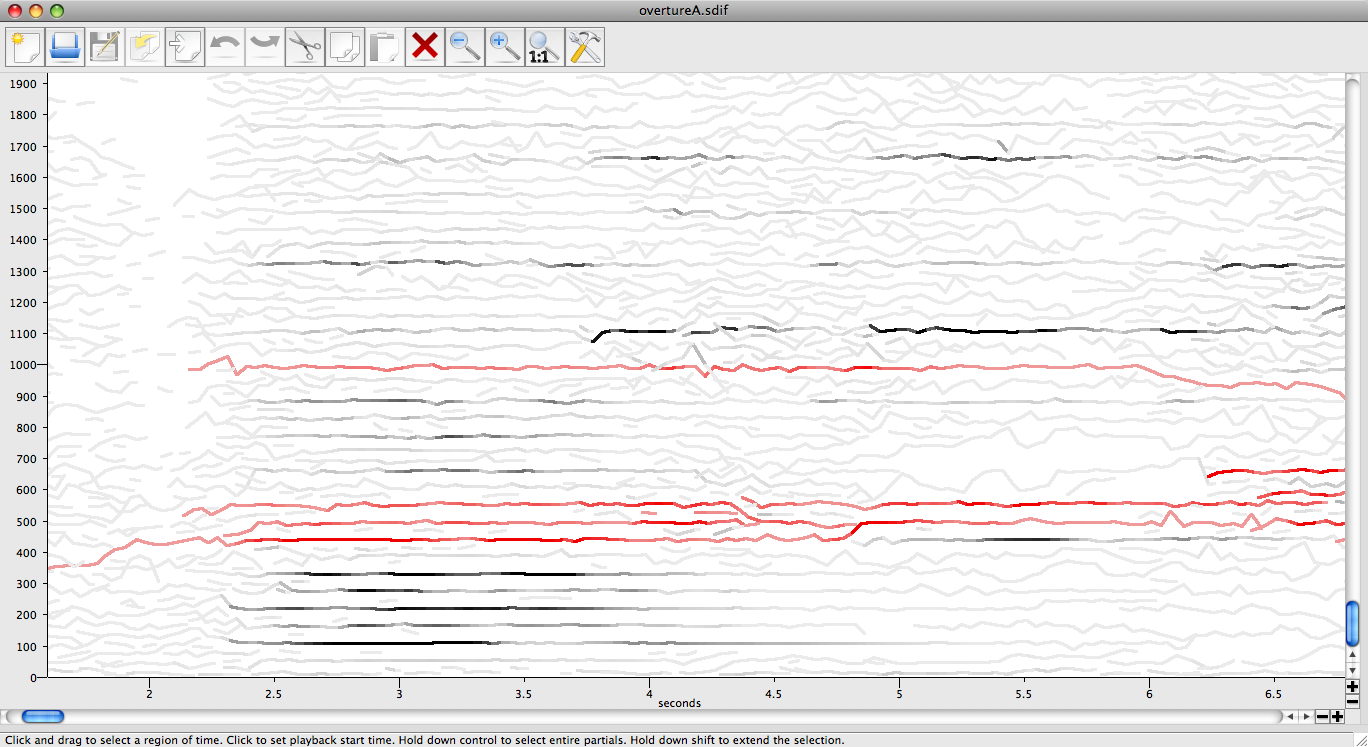
\includegraphics[width=15cm]{Chapter4/Spear1.tif} %change centimeters for resizeing
   \caption{SPEAR graphical interface.}
   \label{fig:example}
\end{figure}
The amplitude and frequency information of each partial given by frame can be stored in a text file. SpearToSC reads text files produced by SPEAR\footnote{SpearToSC reads SPEAR text files in the \emph{Text - Partials} format only.} as a string and strips it into a multidimensional array in SuperCollider. It is therefore possible to process this data within the SuperCollider language and server and re-synthesize this information not only with sinusoidal waves, but with any type of Unit Generator. 

\href{http://github.com/freuben/FedeLib/blob/master/SpearToSC/SpearToMIDI.sc}{SpearToMIDI} is a class that inherits functionality from SpearToSC and reduces the information given by SPEAR to be used as data to produce a MIDI file or to control SuperCollider synthesis definitions. The purpose of this class is to reduce the spectral information to an amount of data that can later produce notated material for a written score, a MIDI file or a control system to be used for triggering synthesis algorithms. The data in the text file generated by SPEAR is available by frame and gives too much information for this purpose. Therefore, SpearToMIDI reduces this data in four stages: First, it takes an amplitude threshold argument which gets rid of all of the partial information that lies bellow this value (as seen in Figure 1.2).
\begin{figure}[htbp] %  figure placement: here, top, bottom, or page
   \centering
   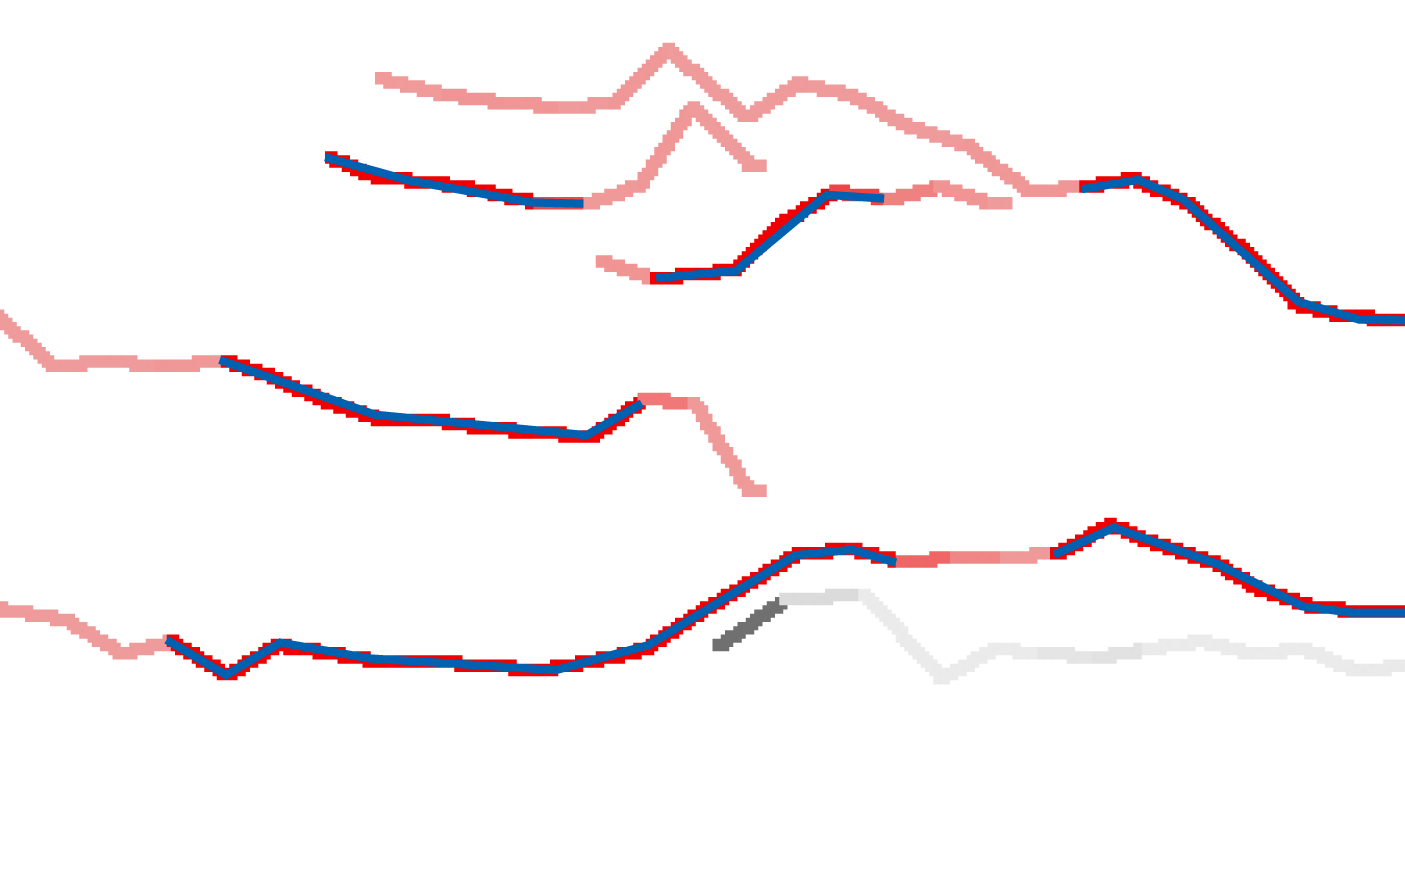
\includegraphics[width=9cm]{Chapter4/Spear2.tif} %change centimeters for resizeing
   \caption{Amplitude threshold selection.}
   \label{fig:example}
\end{figure}\
In other words, it breaks the partial in different groups by introducing silences instead of the data that lies bellow the threshold and at the same time keeps track of the beginning and the end of each group. 

The second stage reduces data with a frequency modulation threshold. Each group is taken as a line and the computer only stores the points in the line which cross a given interval (the modulation threshold). For example, Figure 1.3 shows how the lines representing the groups in Figure 1.2 are traced by selecting the points that cross a given interval.\footnote{The grid represents the intervals as shown in the y-axis. For the purpose of simplification, the diagram doesn't show a logarithmic representation of frequency.} 
\begin{figure}[htbp] %  figure placement: here, top, bottom, or page
   \centering
   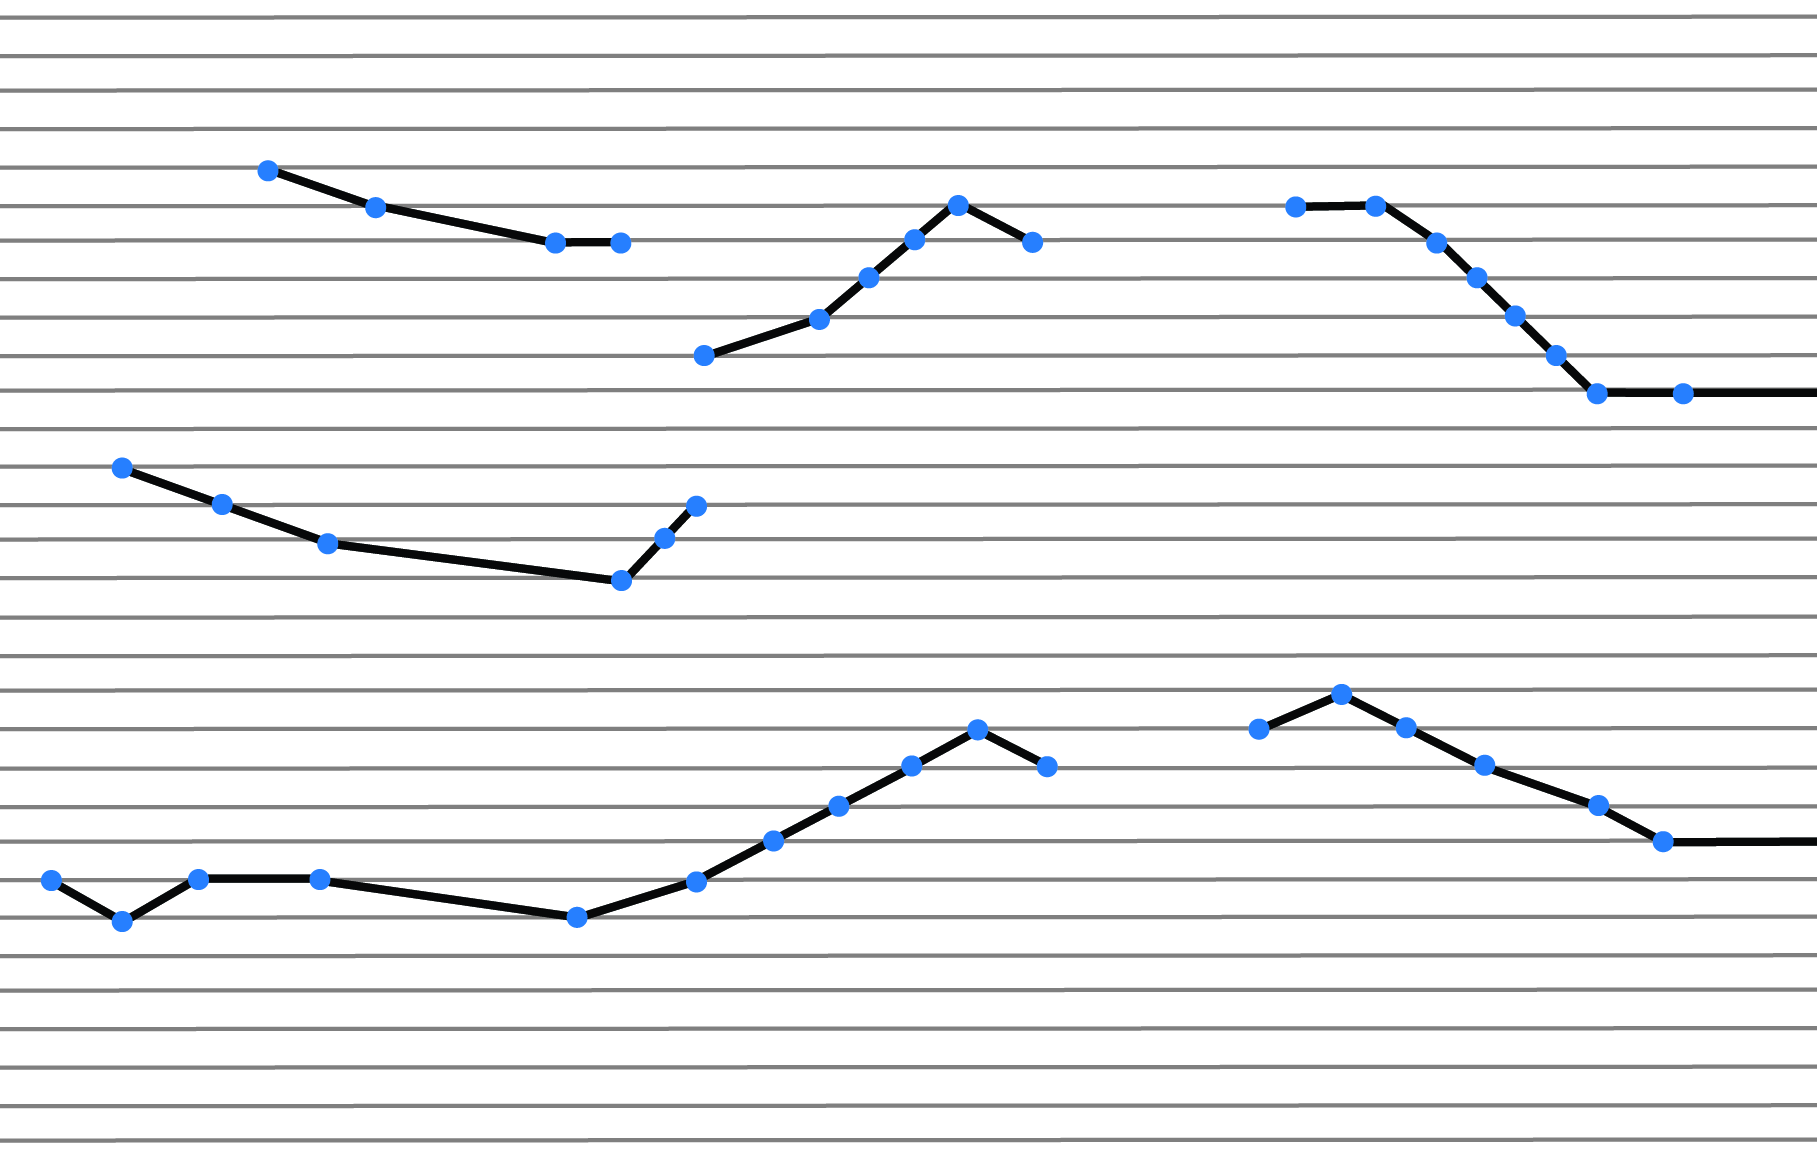
\includegraphics[width=10cm]{Chapter4/Spear3.tif} %change centimeters for resizeing
   \caption{Point selection through frequency modulation threshold.}
   \label{fig:example}
\end{figure}\
If the interval is of one semitone then the frequencies are averaged to the closest chromatic note. It is possible to make microtonal divisions of the equal-tempered scale by using floating point values for the modulation threshold. The magnitude, frequency and time values for each point are stored as a collection of data. This collection can then be accessed and used to control synthesis definitions externally by generating envelopes, which gradually change frequency to produce glissandos and amplitude for gradual volume change. After these first two stages, the original data from Spear is reduced considerably by disregarding details that are not vital for the given purpose. 

The third stage, takes the points of the lines that where obtained in the previous stage and translates them into single notes with a start and an end and that do not change in frequency and amplitude while playing--- in other words, a format that is compatible with the MIDI note-on and note-off paradigm. The points are then considered as representing note-on messages and the note-off messages are calculated depending on whether the point is followed by another new point or if the point is the last of the group, in which case a silence would proceed. In other words, a note-off is inserted before a new note-on or just before a silence. Figure 1.4 
\begin{figure}[htbp] %  figure placement: here, top, bottom, or page
   \centering
   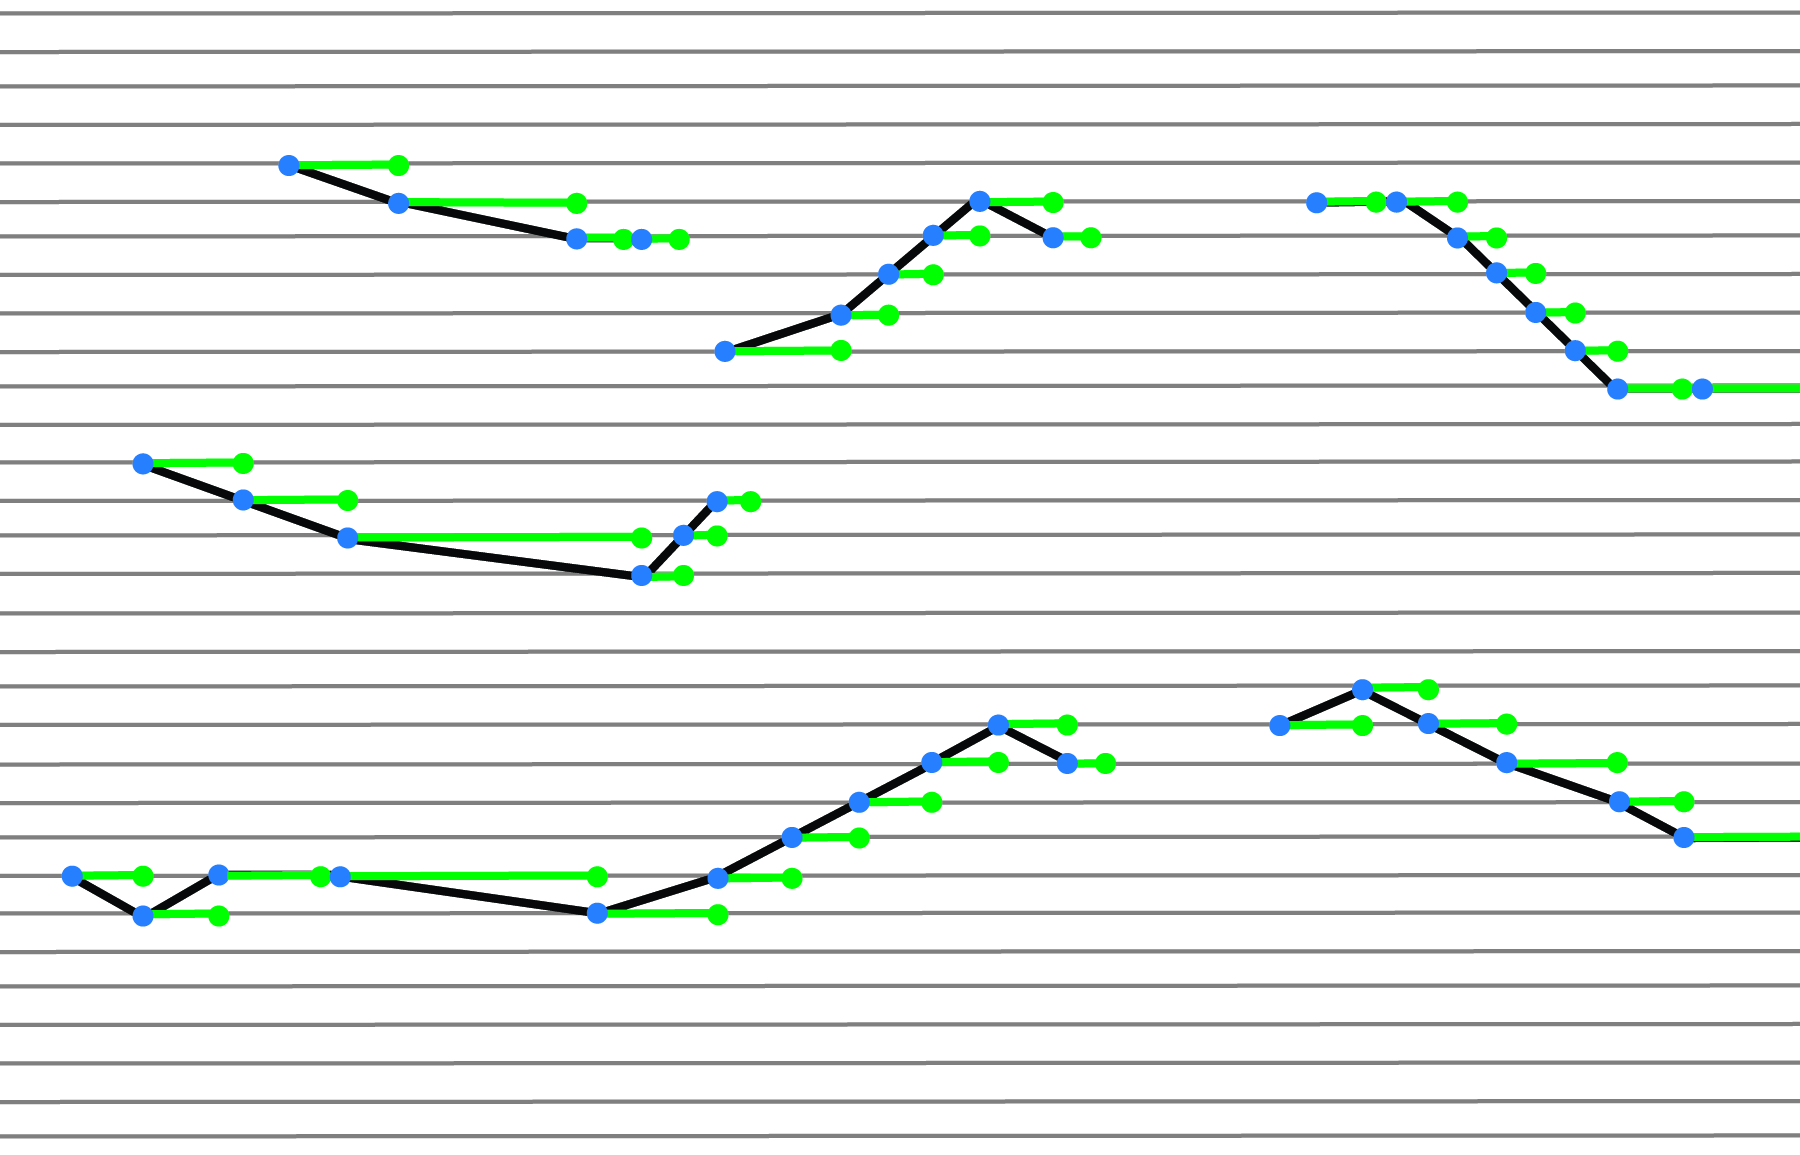
\includegraphics[width=10cm]{Chapter4/Spear4.tif} %change centimeters for resizeing
   \caption{Note representation.}
   \label{fig:example}
\end{figure}\
shows the note representation derived from Figure 1.3, where the notes are seen as green lines, the note-on messages as blue points and the note off messages as green notes. 
The results of this stage can be used to generate a MIDI file\footnote{Using the SimpleMIDIFile class that is part of wslib by \href{http://www.woutersnoei.nl/}{Wouter Snoei}, which is can be obtained as a Quark.} with the intention of either using it to trigger a sampler or to import it into a notation software to create a written score. The user can input the time signature and tempo for the MIDI file as well as an interval value that divides the MIDI note range into different MIDI tracks. By doing this, the notes are separated into different tracks depending on their value in relationship to each other with the purpose of not having too many notes in the same track. Furthermore, these results can be used to create a list of OSC (Open Sound Control) commands that can be sent to the SuperCollider Server for Real-Time-Synthesis and Non-Real-Time-Synthesis. Extra arguments can also be added to control other values in the synthesis definition, which can be set individually by using a function to be evaluated for each instance of the definition.

\section{Real-Time Scoring}

\subsection{AlgorithmicScore}

\section{Pre-compositional Tools}

\subsection{MIDI Mapping}

\subsection{MIDI Triggering}

\label{ch:compamp}